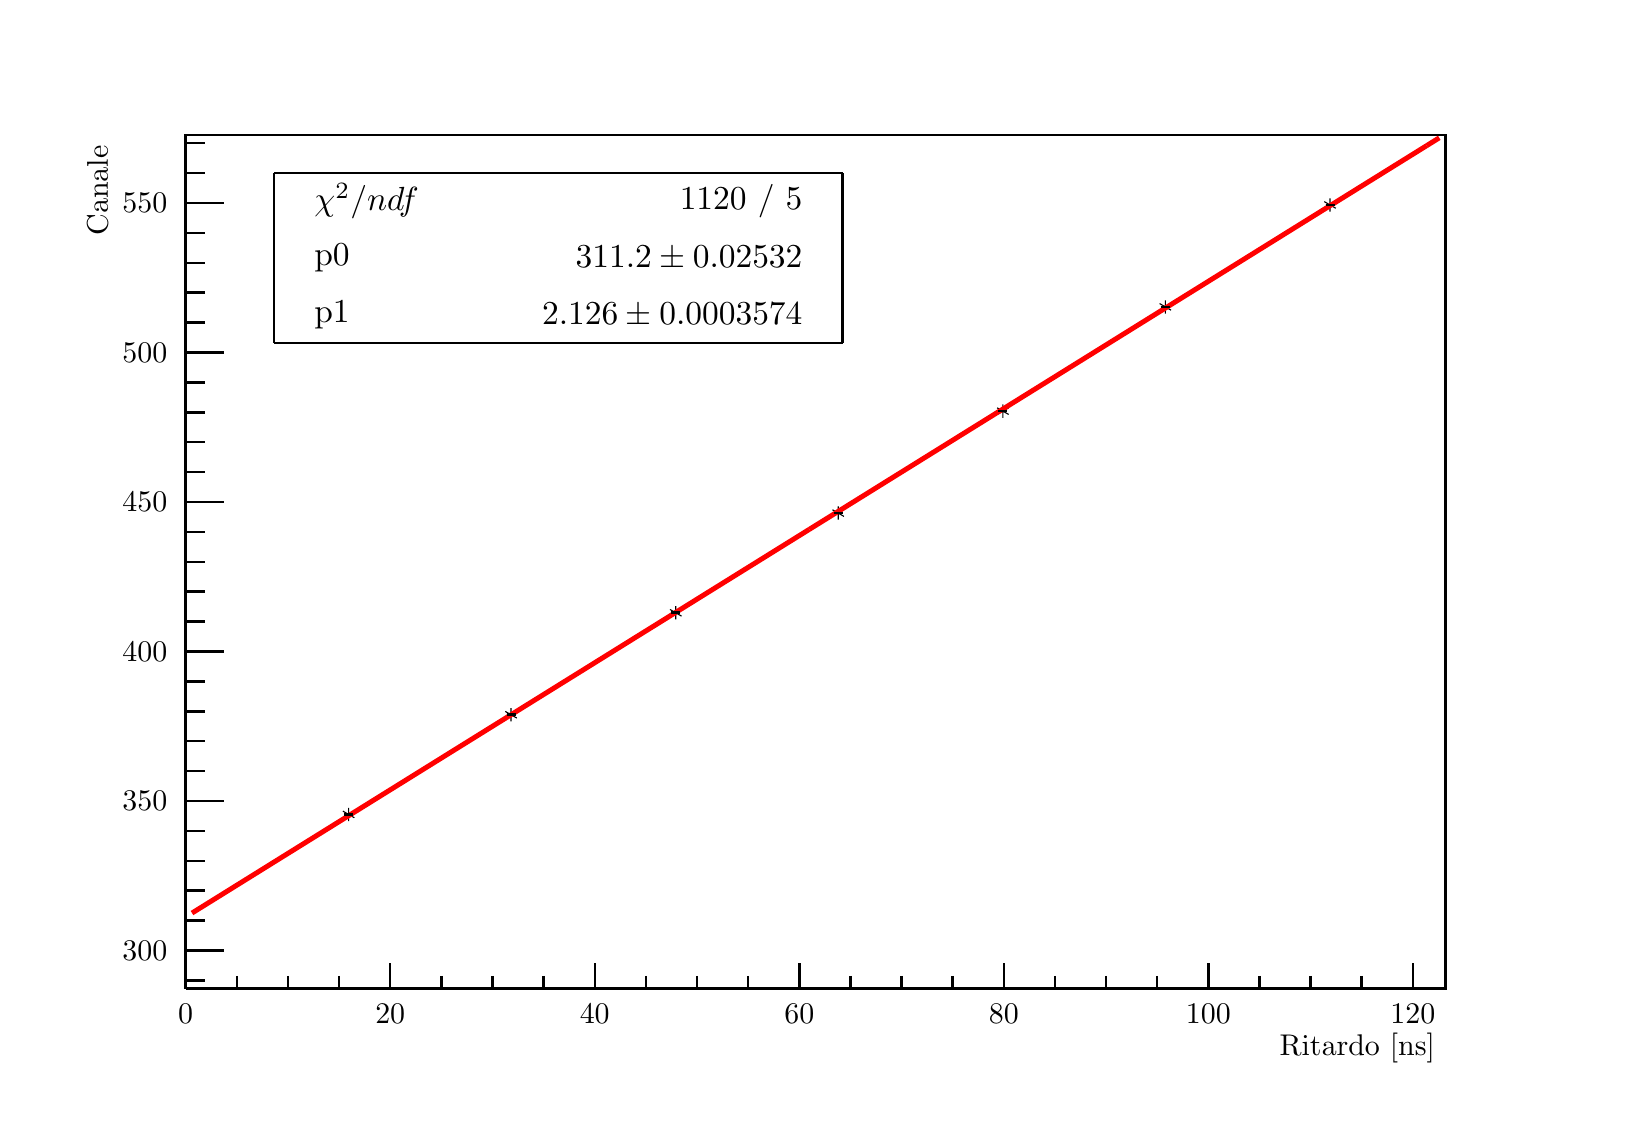
\begin{tikzpicture}
\pgfdeclareplotmark{cross} {
\pgfpathmoveto{\pgfpoint{-0.3\pgfplotmarksize}{\pgfplotmarksize}}
\pgfpathlineto{\pgfpoint{+0.3\pgfplotmarksize}{\pgfplotmarksize}}
\pgfpathlineto{\pgfpoint{+0.3\pgfplotmarksize}{0.3\pgfplotmarksize}}
\pgfpathlineto{\pgfpoint{+1\pgfplotmarksize}{0.3\pgfplotmarksize}}
\pgfpathlineto{\pgfpoint{+1\pgfplotmarksize}{-0.3\pgfplotmarksize}}
\pgfpathlineto{\pgfpoint{+0.3\pgfplotmarksize}{-0.3\pgfplotmarksize}}
\pgfpathlineto{\pgfpoint{+0.3\pgfplotmarksize}{-1.\pgfplotmarksize}}
\pgfpathlineto{\pgfpoint{-0.3\pgfplotmarksize}{-1.\pgfplotmarksize}}
\pgfpathlineto{\pgfpoint{-0.3\pgfplotmarksize}{-0.3\pgfplotmarksize}}
\pgfpathlineto{\pgfpoint{-1.\pgfplotmarksize}{-0.3\pgfplotmarksize}}
\pgfpathlineto{\pgfpoint{-1.\pgfplotmarksize}{0.3\pgfplotmarksize}}
\pgfpathlineto{\pgfpoint{-0.3\pgfplotmarksize}{0.3\pgfplotmarksize}}
\pgfpathclose
\pgfusepathqstroke
}
\pgfdeclareplotmark{cross*} {
\pgfpathmoveto{\pgfpoint{-0.3\pgfplotmarksize}{\pgfplotmarksize}}
\pgfpathlineto{\pgfpoint{+0.3\pgfplotmarksize}{\pgfplotmarksize}}
\pgfpathlineto{\pgfpoint{+0.3\pgfplotmarksize}{0.3\pgfplotmarksize}}
\pgfpathlineto{\pgfpoint{+1\pgfplotmarksize}{0.3\pgfplotmarksize}}
\pgfpathlineto{\pgfpoint{+1\pgfplotmarksize}{-0.3\pgfplotmarksize}}
\pgfpathlineto{\pgfpoint{+0.3\pgfplotmarksize}{-0.3\pgfplotmarksize}}
\pgfpathlineto{\pgfpoint{+0.3\pgfplotmarksize}{-1.\pgfplotmarksize}}
\pgfpathlineto{\pgfpoint{-0.3\pgfplotmarksize}{-1.\pgfplotmarksize}}
\pgfpathlineto{\pgfpoint{-0.3\pgfplotmarksize}{-0.3\pgfplotmarksize}}
\pgfpathlineto{\pgfpoint{-1.\pgfplotmarksize}{-0.3\pgfplotmarksize}}
\pgfpathlineto{\pgfpoint{-1.\pgfplotmarksize}{0.3\pgfplotmarksize}}
\pgfpathlineto{\pgfpoint{-0.3\pgfplotmarksize}{0.3\pgfplotmarksize}}
\pgfpathclose
\pgfusepathqfillstroke
}
\pgfdeclareplotmark{newstar} {
\pgfpathmoveto{\pgfqpoint{0pt}{\pgfplotmarksize}}
\pgfpathlineto{\pgfqpointpolar{44}{0.5\pgfplotmarksize}}
\pgfpathlineto{\pgfqpointpolar{18}{\pgfplotmarksize}}
\pgfpathlineto{\pgfqpointpolar{-20}{0.5\pgfplotmarksize}}
\pgfpathlineto{\pgfqpointpolar{-54}{\pgfplotmarksize}}
\pgfpathlineto{\pgfqpointpolar{-90}{0.5\pgfplotmarksize}}
\pgfpathlineto{\pgfqpointpolar{234}{\pgfplotmarksize}}
\pgfpathlineto{\pgfqpointpolar{198}{0.5\pgfplotmarksize}}
\pgfpathlineto{\pgfqpointpolar{162}{\pgfplotmarksize}}
\pgfpathlineto{\pgfqpointpolar{134}{0.5\pgfplotmarksize}}
\pgfpathclose
\pgfusepathqstroke
}
\pgfdeclareplotmark{newstar*} {
\pgfpathmoveto{\pgfqpoint{0pt}{\pgfplotmarksize}}
\pgfpathlineto{\pgfqpointpolar{44}{0.5\pgfplotmarksize}}
\pgfpathlineto{\pgfqpointpolar{18}{\pgfplotmarksize}}
\pgfpathlineto{\pgfqpointpolar{-20}{0.5\pgfplotmarksize}}
\pgfpathlineto{\pgfqpointpolar{-54}{\pgfplotmarksize}}
\pgfpathlineto{\pgfqpointpolar{-90}{0.5\pgfplotmarksize}}
\pgfpathlineto{\pgfqpointpolar{234}{\pgfplotmarksize}}
\pgfpathlineto{\pgfqpointpolar{198}{0.5\pgfplotmarksize}}
\pgfpathlineto{\pgfqpointpolar{162}{\pgfplotmarksize}}
\pgfpathlineto{\pgfqpointpolar{134}{0.5\pgfplotmarksize}}
\pgfpathclose
\pgfusepathqfillstroke
}
\definecolor{c}{rgb}{1,1,1};
\draw [color=c, fill=c] (0,0) rectangle (20,13.553);
\draw [color=c, fill=c] (2,1.3553) rectangle (18,12.1977);
\definecolor{c}{rgb}{0,0,0};
\draw [c,line width=0.9] (2,1.3553) -- (2,12.1977) -- (18,12.1977) -- (18,1.3553) -- (2,1.3553);
\definecolor{c}{rgb}{1,1,1};
\draw [color=c, fill=c] (2,1.3553) rectangle (18,12.1977);
\definecolor{c}{rgb}{0,0,0};
\draw [c,line width=0.9] (2,1.3553) -- (2,12.1977) -- (18,12.1977) -- (18,1.3553) -- (2,1.3553);
\draw [c,line width=0.9] (2,1.3553) -- (18,1.3553);
\draw [anchor= east] (18,0.596332) node[scale=1.08185, color=c, rotate=0]{Ritardo [ns]};
\draw [c,line width=0.9] (2,1.68057) -- (2,1.3553);
\draw [c,line width=0.9] (2.64935,1.51794) -- (2.64935,1.3553);
\draw [c,line width=0.9] (3.2987,1.51794) -- (3.2987,1.3553);
\draw [c,line width=0.9] (3.94805,1.51794) -- (3.94805,1.3553);
\draw [c,line width=0.9] (4.5974,1.68057) -- (4.5974,1.3553);
\draw [c,line width=0.9] (5.24675,1.51794) -- (5.24675,1.3553);
\draw [c,line width=0.9] (5.8961,1.51794) -- (5.8961,1.3553);
\draw [c,line width=0.9] (6.54545,1.51794) -- (6.54545,1.3553);
\draw [c,line width=0.9] (7.19481,1.68057) -- (7.19481,1.3553);
\draw [c,line width=0.9] (7.84416,1.51794) -- (7.84416,1.3553);
\draw [c,line width=0.9] (8.49351,1.51794) -- (8.49351,1.3553);
\draw [c,line width=0.9] (9.14286,1.51794) -- (9.14286,1.3553);
\draw [c,line width=0.9] (9.79221,1.68057) -- (9.79221,1.3553);
\draw [c,line width=0.9] (10.4416,1.51794) -- (10.4416,1.3553);
\draw [c,line width=0.9] (11.0909,1.51794) -- (11.0909,1.3553);
\draw [c,line width=0.9] (11.7403,1.51794) -- (11.7403,1.3553);
\draw [c,line width=0.9] (12.3896,1.68057) -- (12.3896,1.3553);
\draw [c,line width=0.9] (13.039,1.51794) -- (13.039,1.3553);
\draw [c,line width=0.9] (13.6883,1.51794) -- (13.6883,1.3553);
\draw [c,line width=0.9] (14.3377,1.51794) -- (14.3377,1.3553);
\draw [c,line width=0.9] (14.987,1.68057) -- (14.987,1.3553);
\draw [c,line width=0.9] (15.6364,1.51794) -- (15.6364,1.3553);
\draw [c,line width=0.9] (16.2857,1.51794) -- (16.2857,1.3553);
\draw [c,line width=0.9] (16.9351,1.51794) -- (16.9351,1.3553);
\draw [c,line width=0.9] (17.5844,1.68057) -- (17.5844,1.3553);
\draw [c,line width=0.9] (17.5844,1.68057) -- (17.5844,1.3553);
\draw [anchor=base] (2,0.908052) node[scale=1.08185, color=c, rotate=0]{0};
\draw [anchor=base] (4.5974,0.908052) node[scale=1.08185, color=c, rotate=0]{20};
\draw [anchor=base] (7.19481,0.908052) node[scale=1.08185, color=c, rotate=0]{40};
\draw [anchor=base] (9.79221,0.908052) node[scale=1.08185, color=c, rotate=0]{60};
\draw [anchor=base] (12.3896,0.908052) node[scale=1.08185, color=c, rotate=0]{80};
\draw [anchor=base] (14.987,0.908052) node[scale=1.08185, color=c, rotate=0]{100};
\draw [anchor=base] (17.5844,0.908052) node[scale=1.08185, color=c, rotate=0]{120};
\draw [c,line width=0.9] (2,1.3553) -- (2,12.1977);
\draw [anchor= east] (0.88,12.1977) node[scale=1.08185, color=c, rotate=90]{Canale};
\draw [c,line width=0.9] (2.48,1.83997) -- (2,1.83997);
\draw [c,line width=0.9] (2.24,2.21972) -- (2,2.21972);
\draw [c,line width=0.9] (2.24,2.59947) -- (2,2.59947);
\draw [c,line width=0.9] (2.24,2.97922) -- (2,2.97922);
\draw [c,line width=0.9] (2.24,3.35896) -- (2,3.35896);
\draw [c,line width=0.9] (2.48,3.73871) -- (2,3.73871);
\draw [c,line width=0.9] (2.24,4.11846) -- (2,4.11846);
\draw [c,line width=0.9] (2.24,4.49821) -- (2,4.49821);
\draw [c,line width=0.9] (2.24,4.87796) -- (2,4.87796);
\draw [c,line width=0.9] (2.24,5.2577) -- (2,5.2577);
\draw [c,line width=0.9] (2.48,5.63745) -- (2,5.63745);
\draw [c,line width=0.9] (2.24,6.0172) -- (2,6.0172);
\draw [c,line width=0.9] (2.24,6.39695) -- (2,6.39695);
\draw [c,line width=0.9] (2.24,6.77669) -- (2,6.77669);
\draw [c,line width=0.9] (2.24,7.15644) -- (2,7.15644);
\draw [c,line width=0.9] (2.48,7.53619) -- (2,7.53619);
\draw [c,line width=0.9] (2.24,7.91594) -- (2,7.91594);
\draw [c,line width=0.9] (2.24,8.29569) -- (2,8.29569);
\draw [c,line width=0.9] (2.24,8.67543) -- (2,8.67543);
\draw [c,line width=0.9] (2.24,9.05518) -- (2,9.05518);
\draw [c,line width=0.9] (2.48,9.43493) -- (2,9.43493);
\draw [c,line width=0.9] (2.24,9.81468) -- (2,9.81468);
\draw [c,line width=0.9] (2.24,10.1944) -- (2,10.1944);
\draw [c,line width=0.9] (2.24,10.5742) -- (2,10.5742);
\draw [c,line width=0.9] (2.24,10.9539) -- (2,10.9539);
\draw [c,line width=0.9] (2.48,11.3337) -- (2,11.3337);
\draw [c,line width=0.9] (2.48,1.83997) -- (2,1.83997);
\draw [c,line width=0.9] (2.24,1.46023) -- (2,1.46023);
\draw [c,line width=0.9] (2.48,11.3337) -- (2,11.3337);
\draw [c,line width=0.9] (2.24,11.7134) -- (2,11.7134);
\draw [c,line width=0.9] (2.24,12.0932) -- (2,12.0932);
\draw [anchor= east] (1.9,1.83997) node[scale=1.08185, color=c, rotate=0]{300};
\draw [anchor= east] (1.9,3.73871) node[scale=1.08185, color=c, rotate=0]{350};
\draw [anchor= east] (1.9,5.63745) node[scale=1.08185, color=c, rotate=0]{400};
\draw [anchor= east] (1.9,7.53619) node[scale=1.08185, color=c, rotate=0]{450};
\draw [anchor= east] (1.9,9.43493) node[scale=1.08185, color=c, rotate=0]{500};
\draw [anchor= east] (1.9,11.3337) node[scale=1.08185, color=c, rotate=0]{550};
\definecolor{c}{rgb}{1,1,1};
\draw [color=c, fill=c] (3.12321,9.55329) rectangle (10.3438,11.7114);
\definecolor{c}{rgb}{0,0,0};
\draw [c,line width=0.9] (3.12321,9.55329) -- (10.3438,9.55329);
\draw [c,line width=0.9] (10.3438,9.55329) -- (10.3438,11.7114);
\draw [c,line width=0.9] (10.3438,11.7114) -- (3.12321,11.7114);
\draw [c,line width=0.9] (3.12321,11.7114) -- (3.12321,9.55329);
\draw [anchor= west] (3.48424,11.3517) node[scale=1.20912, color=c, rotate=0]{$\chi^{2} / ndf $};
\draw [anchor= east] (9.98281,11.3517) node[scale=1.20912, color=c, rotate=0]{  1120 / 5};
\draw [anchor= west] (3.48424,10.6323) node[scale=1.20912, color=c, rotate=0]{p0       };
\draw [anchor= east] (9.98281,10.6323) node[scale=1.20912, color=c, rotate=0]{$ 311.2 \pm 0.02532$};
\draw [anchor= west] (3.48424,9.91298) node[scale=1.20912, color=c, rotate=0]{p1       };
\draw [anchor= east] (9.98281,9.91298) node[scale=1.20912, color=c, rotate=0]{$ 2.126 \pm 0.0003574$};
\foreach \P in {(4.06877,3.5681), (6.13181,4.83419), (8.2235,6.12907), (10.2865,7.39517), (12.3782,8.69004), (14.4413,10.0137), (16.5329,11.3086)}{\draw[mark options={color=c,fill=c},mark size=2.402402pt,mark=asterisk] plot coordinates {\P};}
\definecolor{c}{rgb}{1,0,0};
\draw [c,line width=1.8] (2.08,2.31566) -- (2.24,2.4151) -- (2.4,2.51455) -- (2.56,2.614) -- (2.72,2.71345) -- (2.88,2.81289) -- (3.04,2.91234) -- (3.2,3.01179) -- (3.36,3.11123) -- (3.52,3.21068) -- (3.68,3.31013) -- (3.84,3.40958) -- (4,3.50902) --
 (4.16,3.60847) -- (4.32,3.70792) -- (4.48,3.80737) -- (4.64,3.90681) -- (4.8,4.00626) -- (4.96,4.10571) -- (5.12,4.20516) -- (5.28,4.3046) -- (5.44,4.40405) -- (5.6,4.5035) -- (5.76,4.60295) -- (5.92,4.70239) -- (6.08,4.80184) -- (6.24,4.90129) --
 (6.4,5.00073) -- (6.56,5.10018) -- (6.72,5.19963) -- (6.88,5.29908) -- (7.04,5.39852) -- (7.2,5.49797) -- (7.36,5.59742) -- (7.52,5.69687) -- (7.68,5.79631) -- (7.84,5.89576) -- (8,5.99521) -- (8.16,6.09466) -- (8.32,6.1941) -- (8.48,6.29355) --
 (8.64,6.393) -- (8.8,6.49244) -- (8.96,6.59189) -- (9.12,6.69134) -- (9.28,6.79079) -- (9.44,6.89023) -- (9.6,6.98968) -- (9.76,7.08913) -- (9.92,7.18858);
\draw [c,line width=1.8] (9.92,7.18858) -- (10.08,7.28802) -- (10.24,7.38747) -- (10.4,7.48692) -- (10.56,7.58637) -- (10.72,7.68581) -- (10.88,7.78526) -- (11.04,7.88471) -- (11.2,7.98416) -- (11.36,8.0836) -- (11.52,8.18305) -- (11.68,8.2825) --
 (11.84,8.38194) -- (12,8.48139) -- (12.16,8.58084) -- (12.32,8.68029) -- (12.48,8.77973) -- (12.64,8.87918) -- (12.8,8.97863) -- (12.96,9.07808) -- (13.12,9.17752) -- (13.28,9.27697) -- (13.44,9.37642) -- (13.6,9.47587) -- (13.76,9.57531) --
 (13.92,9.67476) -- (14.08,9.77421) -- (14.24,9.87366) -- (14.4,9.9731) -- (14.56,10.0725) -- (14.72,10.172) -- (14.88,10.2714) -- (15.04,10.3709) -- (15.2,10.4703) -- (15.36,10.5698) -- (15.52,10.6692) -- (15.68,10.7687) -- (15.84,10.8681) --
 (16,10.9676) -- (16.16,11.067) -- (16.32,11.1665) -- (16.48,11.2659) -- (16.64,11.3654) -- (16.8,11.4648) -- (16.96,11.5643) -- (17.12,11.6637) -- (17.28,11.7632) -- (17.44,11.8626) -- (17.6,11.962) -- (17.76,12.0615);
\draw [c,line width=1.8] (17.76,12.0615) -- (17.92,12.1609);
\definecolor{c}{rgb}{1,1,1};
\draw [color=c, fill=c] (3.12321,9.55329) rectangle (10.3438,11.7114);
\definecolor{c}{rgb}{0,0,0};
\draw [c,line width=0.9] (3.12321,9.55329) -- (10.3438,9.55329);
\draw [c,line width=0.9] (10.3438,9.55329) -- (10.3438,11.7114);
\draw [c,line width=0.9] (10.3438,11.7114) -- (3.12321,11.7114);
\draw [c,line width=0.9] (3.12321,11.7114) -- (3.12321,9.55329);
\draw [anchor= west] (3.48424,11.3517) node[scale=1.20912, color=c, rotate=0]{$\chi^{2} / ndf $};
\draw [anchor= east] (9.98281,11.3517) node[scale=1.20912, color=c, rotate=0]{  1120 / 5};
\draw [anchor= west] (3.48424,10.6323) node[scale=1.20912, color=c, rotate=0]{p0       };
\draw [anchor= east] (9.98281,10.6323) node[scale=1.20912, color=c, rotate=0]{$ 311.2 \pm 0.02532$};
\draw [anchor= west] (3.48424,9.91298) node[scale=1.20912, color=c, rotate=0]{p1       };
\draw [anchor= east] (9.98281,9.91298) node[scale=1.20912, color=c, rotate=0]{$ 2.126 \pm 0.0003574$};
\draw [c,line width=0.9] (4.06877,3.5681) -- (4.06877,3.56923);
\draw [c,line width=0.9] (4.01146,3.56923) -- (4.12607,3.56923);
\draw [c,line width=0.9] (4.06877,3.5681) -- (4.06877,3.56696);
\draw [c,line width=0.9] (4.01146,3.56696) -- (4.12607,3.56696);
\draw [c,line width=0.9] (6.13181,4.83419) -- (6.13181,4.83533);
\draw [c,line width=0.9] (6.0745,4.83533) -- (6.18911,4.83533);
\draw [c,line width=0.9] (6.13181,4.83419) -- (6.13181,4.83305);
\draw [c,line width=0.9] (6.0745,4.83305) -- (6.18911,4.83305);
\draw [c,line width=0.9] (8.2235,6.12907) -- (8.2235,6.13021);
\draw [c,line width=0.9] (8.16619,6.13021) -- (8.2808,6.13021);
\draw [c,line width=0.9] (8.2235,6.12907) -- (8.2235,6.12793);
\draw [c,line width=0.9] (8.16619,6.12793) -- (8.2808,6.12793);
\draw [c,line width=0.9] (10.2865,7.39517) -- (10.2865,7.39631);
\draw [c,line width=0.9] (10.2292,7.39631) -- (10.3438,7.39631);
\draw [c,line width=0.9] (10.2865,7.39517) -- (10.2865,7.39403);
\draw [c,line width=0.9] (10.2292,7.39403) -- (10.3438,7.39403);
\draw [c,line width=0.9] (12.3782,8.69004) -- (12.3782,8.69156);
\draw [c,line width=0.9] (12.3209,8.69156) -- (12.4355,8.69156);
\draw [c,line width=0.9] (12.3782,8.69004) -- (12.3782,8.68852);
\draw [c,line width=0.9] (12.3209,8.68852) -- (12.4355,8.68852);
\draw [c,line width=0.9] (14.4413,10.0137) -- (14.4413,10.0148);
\draw [c,line width=0.9] (14.384,10.0148) -- (14.4986,10.0148);
\draw [c,line width=0.9] (14.4413,10.0137) -- (14.4413,10.0125);
\draw [c,line width=0.9] (14.384,10.0125) -- (14.4986,10.0125);
\draw [c,line width=0.9] (16.5329,11.3086) -- (16.5329,11.3097);
\draw [c,line width=0.9] (16.4756,11.3097) -- (16.5903,11.3097);
\draw [c,line width=0.9] (16.5329,11.3086) -- (16.5329,11.3074);
\draw [c,line width=0.9] (16.4756,11.3074) -- (16.5903,11.3074);
\end{tikzpicture}
